\documentclass[a4paper,11pt]{article}

% ***********************************************************
%    comment this line for creating the submission version
% ***********************************************************
\def\InternRev{}

\usepackage{float}
\usepackage{lastpage}
\usepackage{titling}
\usepackage{authblk}
\usepackage{lipsum}

\renewcommand\Affilfont{\footnotesize}

\usepackage[utf8]{inputenc}
\usepackage[textfont={},labelfont={bf},format=plain,labelsep=space]{caption}
\usepackage[top=2.5cm,bottom=2.5cm,outer=2.5cm,inner=2.0cm]{geometry}
\usepackage{amssymb}
\usepackage{amsmath}
\usepackage{graphicx}

\usepackage{helvet}
\renewcommand{\familydefault}{\sfdefault}

% tables
\usepackage{booktabs}
\usepackage{adjustbox}
\usepackage{threeparttable}
\usepackage{multirow}


\usepackage[binary-units=true]{siunitx}
\sisetup{
	separate-uncertainty,
	table-align-uncertainty = true
}
\DeclareSIUnit\pixel{pixel}
\DeclareSIUnit\fps{fps}
\DeclareMathOperator*{\argmin}{\arg\!\min}
\newcommand*{\norm}[1]{\left\lVert#1\right\rVert}

\usepackage[super]{nth}

\setlength{\parindent}{1.5em}

\usepackage{setspace}

\usepackage{hyperref}
\hypersetup{
	colorlinks=false,
	urlcolor=cyan,
}
\urlstyle{same}

\usepackage[capitalise,noabbrev]{cleveref}
\usepackage[numbers,sort&compress]{natbib}
\bibliographystyle{vancouver-authoryear}
\renewcommand{\refname}{REFERENCES}
\renewcommand{\bibname}{REFERENCES}



% for review
\usepackage{xcolor}
\newcommand{\hlequ}[1]{\colorbox{yellow!50}{$\displaystyle#1$}}
\usepackage{soul}


\usepackage{titlesec}
\titleformat{\section}{\bfseries\Large}{\thesection}{1em}{}
\titleformat{\subsection}{\bfseries\large}{\thesubsection}{1em}{}
\titleformat{\subsubsection}{\bfseries}{\thesubsubsection}{1em}{}
\renewcommand{\thesection}{\arabic{section}}

% for equations that is longer than 1 line
\newcommand{\splitatcommas}[1]{%
	\begingroup
	\begingroup\lccode`~=`, \lowercase{\endgroup
		\edef~{\mathchar\the\mathcode`, \penalty0 \noexpand\hspace{0pt plus 1em}}%
	}\mathcode`,="8000 #1%
	\endgroup
}



\title{Stack-of-Radial Echo Planar Imaging \\with Locally Low Rank Regularized Subspace Reconstruction \\
	for Fast High-Resolution Brain MRI}
% \date{\vspace{-5ex}} % no date on the title page

\author[1]{Zhengguo Tan}
\author[2]{Erpeng Dai}
\author[3,4]{Martin Uecker}

% Include full affiliation details for all authors
\affil[1]{Department Artificial Intelligence in Biomedical Engineering, Friedrich-Alexander-Universit\"at Erlangen-N\"urnberg, Erlangen, Germany}
\affil[2]{Department of Radiology, Stanford University, Stanford, CA, 94305, United States}
\affil[3]{Institute of Biomedical Imaging, Graz University of Technology, Graz, Austria}
\affil[4]{Institute for Diagnostic and Interventional Radiology, University Medical Center G\"ottingen, G\"ottingen, Germany}



\begin{document}
\maketitle
\vfill

\begin{flushleft}

\textbf{Note:}\\
Part of this article was presented at the Joint Annual Meeting ISMRM-ESMRMB
\& ISMRT \nth{31} Annual Meeting, London, United Kingdom, 2022.

\vspace*{1.0\baselineskip}

\textbf{Correspondence to:}\\
Dr.~Zhengguo Tan\\
Department Artificial Intelligence in Biomedical Engineering\\
Friedrich-Alexander-Universit\"at Erlangen-N\"urnberg\\
Werner-von-Siemens-Str. 61\\
91052 Erlangen, Germany\\
Email: zhengguo.tan@fau.de

\vspace*{1.0\baselineskip}

\textbf{Funding information:}\\
DFG (German Research Foundation): TA 1473/2-1, UE 189/4-1, EXC 2067/1-390729940. \\
NIH (National Institutes of Health): U24EB029240.

\vspace*{1.0\baselineskip}

\textbf{Running head:} \\
Volumetric Radial EPI

\vspace*{1.0\baselineskip}

Number of Pages: \pageref{LastPage}\\
Number of Figures: 5\\
Number of Supporting Figures: 3\\
Number of Supporting Videos: 1\\
Number of References: 31\\
Number of Words: 228 (abstract); $\mathtt{\sim}$2327 (body)

\vspace*{1.0\baselineskip}

Submitted to \textit{Magnetic Resonance in Medicine as Technical Note}\\
	
\end{flushleft}

\pagebreak


\doublespacing

% =============================================== %
% 		abstract page
% =============================================== %
\noindent
\textbf{Purpose:} To develop stack-of-radial echo planar imaging (EPI) 
with linear subspace reconstruction for volumetric, fast, and high-resolution 
brain magnetic resonance imaging (MRI).\\
\textbf{Methods:} We implemented the stack-of-radial EPI 
sequence for in vivo brain acquisition. 
The acquisition protocol employed flow flip angle (4~degree) excitation 
without fat saturation, 
covered the whole brain with 192 slices per volume, 
and utilized only 7 excitation per slice 
with an echo train length of 35. 
This allowed for fast and high-resolution brain MRI 
with \SI{1}{\mm} isotropic resolution in \SI{1.3}{\minute}. 
For image reconstruction, 
we leveraged the linear subspace modeling method 
of the acquired multi-gradient-echo (MGRE) signal 
by constructing the truncated-SVD subspace matrix from the simulated dictionary. 
The subspace coefficient maps with respect to the subspace matrix were then 
iteratively reconstructed with locally low rank (LLR) regularization. \\
\textbf{Results:} We numerically and experimentally demonstrated that 
a large number of subspace coefficients were required to accurately 
represent the MGRE signal with off-resonance induced rapid phase modulation. 
In vivo brain results showed no spatial distortion artifacts in radial EPI. 
Excellent $T_2^*$ contrast in the echo-combined images 
throughout the whole brain was achieved. 
Residual streaks existed likely due to the lack of proper reference scans.\\
\textbf{Conclusion:} The proposed volumetric radial EPI 
with advanced LLR regularized linear subspace reconstruction 
achieved fast and high spatial resolution brain MRI. 
This preliminary results showed promises for 
various potential brain MRI applications.

\vspace*{3.0\baselineskip}
\noindent 
\textbf{KEYWORDS} \\
Linear Subspace,
Locally low rank,
Radial MRI,
Echo Planar Imaging,
Brain MRI.

\vfill
\pagebreak


% =============================================== %
% 		introduction
% =============================================== %
\section{INTRODUCTION}

Echo planar imaging (EPI) \cite{mansfield_1977_epi} is 
an ultra fast and effective imaging technique, 
characterized by long echo train readouts per radio frequency excitation and 
the formation of an image from one single or a couple of excitation.
Therefore, EPI has been used in various MRI applications, 
e.g.~functional \cite{ogawa_1990_fmri}, diffusion \cite{lebihan_1986_diff}, 
and arterial spin labeling imaging \cite{feinberg_2013_asl}. 

Although fast, the conventional EPI technique is limited to relatively 
low spatial resolution and suffers from spatial distortion artifacts 
due to off resonances. 
Recent progress in echo planar time resolved imaging (EPTI) 
using either combined gradient and spin echoes (GRASE) 
or multiple gradient echoes (MGRE) has achieved simultaneous 
multi-slice multi-parameter mapping in high spatio-temporal resolution 
\cite{wang_2019_epti}. 
The EPTI sequence is a multi-shot segmented multi-echo sampling method. 
It explores complementary sampling patterns 
among echoes as well as among shots and recovered multi-echo images 
via tilted-CAIPI reconstruction \cite{dong_2019_tilted_capi}. 
Further progress in 3D EPTI and linear subspace reconstruction 
has achieved \SI{1}{\mm} isotropic resolution and 210 slices coverage 
in about three minutes \cite{dong_2021_vfa_epti}. 
However, the local-patch-wise sampling of the $k_y$-$k_z$ plane 
requires dedicated shot-to-shot $B_0$ variation correction algorithms.

Beside Cartesian-based EPI/EPTI techniques, 
radial EPI has also been proposed. 
One appealing feature of radial EPI is its immunity to 
spatial distortion artifacts \cite{silva_1998_repi}, 
but early developments 
\cite{seifert_2000_rtse,theilmann_2004_vo_rfse,jung_2009_rssfp,lee_2010_repi,bhat_2011_repi_heart} 
achieved relatively short echo train length (i.e.~smaller than 5), 
thereby limiting its sampling speed.
Recently, Rettenmeier et al.~\cite{rettenmeier_2021_repi} proposed 3D 
twisted radial EPI for functional brain MRI, 
where echo trains along the $k_z$ direction were rotated (twisted) 
to promote incoherent $k_z$ undersampling. 
Image reconstruction was then based on 
the CG-SENSE algorithm \cite{pruessmann_2001_gsense} with a pre-calibrated 
$B_0$ inhomogeneity \cite{funai_2008_secondorder} as well as 
coil sensitivities maps \cite{walsh_2000_coil}. 
Although promising, this technique requires 
large blip gradients to traverse among slices.

To explore the sampling efficiency of radial sampling 
and to develop fast high-resolution brain imaging methods, 
this work proposed the $k_x$-$k_y$-plane radial EPI readouts 
\cite{tan_2016_phd,tan_2019_mobawf} 
combined with 3D stack-of-stars $k_z$ sampling \cite{block_2014_rad} 
for \SI{1}{\mm} isotropic brain imaging. 
Further, the advantage of the complementary sampling pattern 
in the $k_x$-$k_y$ plane is exploited 
with the use of 
linear subspace modeling \cite{huang_2012_t2basis,tamir_2017_t2shuffling} 
and locally low rank (LLR) regularized reconstruction \cite{zhang_2015_llr}.

% =============================================== %
% 		methods
% =============================================== %
\section{METHODS}

\subsection*{Radial EPI Experiments}

In vivo brain MRI experiments on four young healthy adults were performed at \SI{3}{\tesla}
(Skyra, Siemens Healthineers, Erlangen, Germany) with a 20-channel head coil.
Written informed consents were obtained from all subjects before MRI experiments 
in compliance with the regulations established by the local ethics committee.

Details about our implemented sequence please refer to 
Supporting Information Figures S1 and S2. 
Similar to the original stack-of-stars sequence \cite{block_2014_rad}, 
we employed slice-selection gradients to loop over all partitions in the $k_z$ direction, 
whereas radial EPI readouts were performed in the $k_x$-$k_y$ plane.
In addition, the standard random-RF (radio frequency) 
and gradient spoiling scheme was used.

Volumetric brain scans were conducted with 1~\si{\cubic\mm} isotropic resolution.
Detailed imaging parameters were: 
flip angle 4 degree with RF bandwidth time product of 10, 
in-plane field-of-view is 220~$\times$~220~\si{\square\mm}, 
base resolution 220, image matrix size 220~$\times$~220, 
a total of 192 slices, bandwidth 840~\si{\Hz \per \pixel}, 
7 excitation per partition, 
35 echoes per excitation with TE ranging from 1.70 to 55.7~ms 
(echo spacing of 1.52~\si{\ms}) and TR 57.4~ms. 
Total scan time was 1.3~minutes. 
No fat saturation pulse was used before RF excitation.
No $k_z$ undersampling \cite{feng_2016_vdGRASP} was employed in this work. 


\subsection*{Linear Subspace Modeling and Reconstruction}

The acquired MGRE signal follows:
\begin{equation}
	s_m = \rho \cdot e^{- \text{TE}_m / T_2^*} \cdot e^{i 2\pi f_{B_0} \text{TE}_m}
	\label{EQU:mgre_signal}
\end{equation}
where $\rho$ is $T_1$-weighted signal intensity at the echo time of \SI{0}{ms},
$T_2^*$ refers to the decay of transversal magnetization caused by 
a combination of spin-spin relaxation and magnetic field inhomogeneity, 
and $f_{B_0}$ is the off-resonance frequency. 
$\text{TE}_m$ is the echo time of the $m$th echo.

This work leveraged the linear subspace representation of the MGRE signal. 
In the MGRE signal simulation, $\rho$ was kept as 1, 
with a total number of $N_\rho = 1$ atom. 
$T_2^*$ linearly varied between $1$ and \SI{200}{ms}, 
with a total number of $N_{T_2^*} = 100$ values.
$f_{B_0}$ was also linearly varying with a total number of $N_{f_{B_0}} = 101$ values, 
but its minimal and maximal values were changed to 
demonstrate the effects of $f_{B_0}$ range on MGRE signal representation.

Therefore, the shape of the simulated dictionary is 
$[N_\text{TE},~ N_\rho,~ N_{T_2^*},~ N_{f_{B_0}}]$. 
We reshaped such a dictionary to two dimensional: 
$[N_\text{TE},~ N_\rho \times N_{T_2^*} \times N_{f_{B_0}}]$ 
and denoted it as matrix $D$. 
Singular value decomposition (SVD) yields:
\begin{equation}
	D = U \Sigma V^*
\end{equation}
where the complex unitary matrix $U$ has the shape $[N_\text{TE},~ N_\text{TE}]$
and can be truncated to its first $K$ ($K \leq N_\text{TE}$) columns, 
denoted as $\hat{U}$ with the shape $[N_\text{TE},~ K]$. 
Thus, the recovered echo signal is 
$\tilde{D} = \hat{U} \times \hat{U}^T \times D$. 
In this work, we iteratively increased $K$ 
such that the resulting $\tilde{D}$ satisfied 
$\frac{\norm{D - \tilde{D}}}{\norm{D}} \leq 10^{-5}$.

With the truncated subspace matrix $\hat{U}$, the linear subspace coefficient maps ($\alpha$)
can be reconstructed via solving
\begin{equation}
	\argmin_\alpha \norm{y - \mathcal{F}_u S \hat{U} \alpha}_2^2 + \lambda R(\alpha) \; .
	\label{EQU:CostFunc}
\end{equation}
$y$ is the measured multi-channel multi-echo $k$-space data. 
$\mathcal{F}_u$ is the non-uniform FFT (NUFFT) 
\cite{fessler_2003_nufft,beatty_2005_nufft}, which varies among echoes.
$S$ is one set of coil sensitivity maps, 
which were estimated via the nonlinear inverse reconstruction for parallel imaging 
using the first echo $k$-space data \cite{uecker_2008_nlinv}. 
The second term in \cref{EQU:CostFunc} corresponds to regularization, 
in which $\lambda$ is the regularization strength (set as $0.001$), 
and $R(\alpha)$ is the locally low rank soft thresholding. 
Therefore, the coefficient maps $\alpha$ has the shape of $[N_x, N_y, K]$ 
with $N_x$ and $N_y$ the image size (i.e.~base resolution).

The simulation of MGRE dictionary and 
the construction of the subspace matrix ($\hat{U}$) 
were performed in Python.
The linear subspace reconstruction with LLR regularization 
were solved with The alternating direction method of multipliers (ADMM) 
\cite{boyd_2010_admm} in Berkeley Advanced Reconstruction Toolbox (BART) 
\cite{uecker_2015_bart}. 
Afterwards, the echo images can be obtained via matrix multiplication 
$\rho = \hat{U} \alpha$, and then the echo-combined image 
can be computed via the root sum square (RSS) of all echo images.
All reconstructions were done on Intel Xeon Gold 6132 CPU, 
and the reconstruction was executed in a slice-by-slice manner, 
i.e.~sequentially. This is possible with a slice FFT along the $k_z$ direction 
of the acquired 3D $k$-space data \cite{feng_2014_grasp}. 
For comparison, adjoint NUFFT with density compensation reconstruction 
of every echo was also performed with subsequent RSS operation 
on the coil and the echo dimensions. 


% =============================================== %
% 		results
% =============================================== %
\section{RESULTS}

\subsection*{Linear Subspace Modeling}

\cref{FIG:SubspaceSim} depicts the representative results of 
linear subspace modeling on MGRE signal in \cref{EQU:mgre_signal}. 
\cref{FIG:SubspaceSim} (A) shows that when increasing the range 
of $B_0$ off-resonance frequencies in the dictionary 
but keeping the number of atoms consistent as 101, 
larger $K$ (i.e.~more subspace coefficients) is required 
such that the relative error between the recovered signal and 
the dictionary is small enough.
\cref{FIG:SubspaceSim} (B) demonstrates that 
the subspace of the dictionary with maximal $|B_0|$ as \SI{50}{\Hz} 
cannot represent the simulated signal with \SI{100}{\Hz} off-resonance frequency. 
On the other hand, when increasing the maximal $|B_0|$ in the dictionary 
gradually toward \SI{100}{\Hz}, 
the subspace recovered signal gets closer toward the simulated signal.

Moreover, another feature of subspace modeling is the capability of 
representing multi compartment signal. 
As shown in \cref{FIG:SubspaceSim} (C), 
a summation of three species with different proton density, $T_2^*$, 
and off-resonance frequencies is simulated. 
The signal recovered by linear subspace modeling 
(with a maximal $|B_0|$ as 100~\si{\Hz} in the dictionary and 31 subspace coefficients) 
matches well with the simulated signal.

\subsection*{Linear Subspace Reconstruction}

\cref{FIG:BasisCoef} displays three representative subspace coefficient maps 
from the LLR regularized linear subspace reconstruction. 
Since no fat saturation pulse was used in the radial EPI acquisition, 
the later coefficient maps (e.g.~the \nth{27}) contained mainly the tissue 
with large off-resonance frequencies. 
Plus, we also observe that the phase modulation 
induced by large off-resonance frequencies 
resulted in residual streaking artifacts 
in the \nth{11} coefficient map, appearing in the frontal brain region.

\cref{FIG:3DBrain} shows the echo-combined images from there different slices 
in the transversal, sagittal, and coronal orientation, respectively.
Firstly, our experimental results show no spatial distortion artifacts 
in radial EPI acquisition. 
Secondly, the major artifacts in radial EPI appear as 
radial streaks and signal void, 
as shown in the first slice of the transversal and the coronal views. 
Thirdly, the volumetric acquisition, 
with the use of low flip angle and long echo-train readout stack-of-radial EPI, 
leads to excellent $T_2^*$ image contrast. 
We also appreciate the clear visibility of cerebral venous, 
as shown in the second slice of the sagittal view.

Please refer to Supporting Information Video S1 
for the visualization of all 192 echo-combined images 
with \SI{1}{\cubic\mm} isotropic spatial resolution and 
a total acquisition time of only \SI{1.3}{\minute} 
in three orthogonal orientations, 
i.e.~transversal, sagittal, and coronal views. 
To appreciate the advantage of the LLR regularized 
linear subspace reconstruction, 
please refer to Supporting Information Figure S3 
for the adjoint NUFFT reconstruction results.

\cref{FIG:BasisSize} compares the linear subspace reconstruction results 
from $K=5$ and $K=31$ in the truncated matrix $\hat{U}$, respectively. 
The $|B_0|$ range was kept consistent as 100~\si{\Hz} and 
a total of 101 $B_0$ atoms in the dictionary. 
This experiment demonstrates that a small $K$ cannot fully represent the signal, 
and thus results in not-converged image reconstruction.

On the other hand, in line with the simulation results in \cref{FIG:SubspaceSim}, 
this experimentally confirms that larger $K$ was necessary 
in the case of wide-range phase modulation in the dictionary of MGRE signal. 
The reconstruction time per slice for $K = 5$ and $K = 31$ 
was about \num{24} and \SI{140}{\second}, respectively. 
The increase of reconstruction time for larger $K$ is expected, 
because larger $K$ basically means more unknowns 
in the reconstructed $\alpha$ maps.

Noteworthy, the reconstructed image with $K = 31$ 
in the first column of \cref{FIG:BasisSize} is free 
of spatial distortion artifacts. 
Such an imaging slice is prone to spatial distortion and signal void 
in the conventional EPI technique, because of its spatial proximity to 
ear and nose canals filled with air. 
Signal void is alleviated in this case via the echo combination operation, 
which performs RSS of all echoes 
and thus avoids signal dropouts due to phase modulation.

\cref{FIG:Echoes} shows the magnitude and phase images 
of the \nth{1}, \nth{10}, and \nth{20} echoes, respectively. 
The LLR regularized linear subspace reconstruction was performed with 
the same dictionary as in \cref{FIG:BasisSize} and $K = 31$. 
Beside $T_2^*$ signal decay, we also observe rapid phase change 
due to $B_0$ off-resonance phase modulation. 
Residual streaking artifacts are visible, especially in the region 
surrounding the skull.

% =============================================== %
% 		discussion
% =============================================== %
\section{DISCUSSION}

The stack-of-radial EPI sequence presents an efficient radial sampling 
for fast high-resolution MRI and has the potential for other imaging modalities, 
e.g.~functional and diffusion MRI. 
This work focused on its use for fast and high resolution $T_2^*$-weighted brain MRI. 
Key features of the stack-of-radial EPI trajectory are 
segmented radial EPI readouts in the $k_x$-$k_y$ plane with seven shots 
and stack-of-stars \cite{block_2014_rad} excitation for isotropic spatial resolution.
This sequence shows potential applicability to other imaging modalities, 
e.g.~diffusion tensor imaging and quantitative susceptibility mapping.

Another feature of this work is the use of linear subspace modeling and 
LLR regularized iterative reconstruction. 
Adequate number of subspace coefficients presents accuracy approximation 
of the MGRE signal. LLR regularization is demonstrated well suited for 
multi-contrast images. 
However, the work required large number of subspace coefficients. 
The number of subspace coefficients can be reduced via 
incorporating the phase modulation term ($\Phi = e^{i2\pi f_{B_0} \text{TE}_m}$) 
into the forward model in \cref{EQU:CostFunc}, 
i.e.~$F(\alpha) = \mathcal{F}_u S \Phi \hat{U} \alpha$ 
\cite{dong_2020_epti_sub}. 
Here, the field inhomogeneity map ($f_{B_0}$) has the shape $[N_x, N_y]$
is pre-calibrated using reference scans. 
This approach is advantageous to reduce 
the number of subspace coefficients, the model complexity, 
and the image reconstruction time. 
Therefore, it would be beneficial to employ reference scans 
for the stack-of-radial EPI acquisition as well.

Compared with the adjoint NUFFT reconstruction in Supporting Information Figure S3, 
streaking artifacts in echo-combined images have been 
largely reduced with the LLR regularized linear subspace reconstruction. 
However, residual streaks are still visible in 
the subspace coefficient maps (\cref{FIG:BasisCoef})
and the individual echo images (\cref{FIG:Echoes}). 
These artifacts might be mitigated via the incorporation of 
fat saturation pulse as well as proper reference scans 
for the coil sensitivity and $B_0$ maps.

The achieved acceleration per echo in this work 
is $0.5 \pi N_{\text{br}} / N_\text{shot} = 0.5\pi \times 220 / 7 \approx 49$. 
Here, $N_\text{br}$ and $N_\text{shot}$ is the base resolution and 
the number of shots per frame, respectively. 
Such high acceleration factor is achievable with the use of blip gradients. 
blip gradients allow for the sampling of different echoes per shot 
(see Supporting Information Figure S1 and S2), 
thereby forming a complementary sampling pattern among echoes. 

In line with the standard stack-of-stars sequence \cite{block_2014_rad}, 
this radial EPI sequence utilizes aligned sampling pattern along the $k_z$ direction. 
In other words, every TR block is repeated for all $k_z$ partitions 
until the next TR with different segment of radial spokes 
(see Supporting Information Figure S1). 
Therefore, one potential direction would be 
to explore complementary $k_z$ sampling patterns 
to further acceleration 3D acquisition.

Another limitation in this work is the relatively large echo spacing (\SI{1.52}{\ms}). 
For EPI-type acquisition, it would be beneficial to reduce the echo spacing to about 
\SI{1}{\ms} \cite{dong_2020_epti_sub}. 
shorter echo spacing can accelerate echo acquisition and reduce 
susceptibility artifacts. Therefore, it would be logic to identify 
contributing factors in the sequence which constraint the bandwidth 
as well as the echo spacing.


% =============================================== %
% 		conclusion
% =============================================== %
\section{CONCLUSION}

We propose a fast and high-resolution brain MRI method that 
combined stack-of-radial radial EPI for volumetric acquisition 
with advanced LLR regularized linear subspace reconstruction. 
Our developed radial EPI sequence exploits complementary sampling 
patterns among echoes in the $k_x$-$k_y$ plain, 
whereas for 3D acquisition radial spoke segments of every shot are 
aligned along the $k_z$ direction. 
LLR regularization presents an effective method for multi-contrast 
image reconstruction.

% =============================================== %
% 		open research
% =============================================== %
\section*{OPEN RESEARCH}

In the spirit of reproducible and open research, 
the proposed method is made openly available as part of BART 
\footnote{\url{https://github.com/mrirecon/bart/}}.
Scripts and data to reproduce the experiments will be made public 
upon the publication of the manuscript.

% =============================================== %
% 		acknowledgment
% =============================================== %
\section*{Acknowledgment}

The authors thank Prof.~Dr.~Florian Knoll for proofreading the paper.

\vfill
\pagebreak

% =============================================== %
% 		references
% =============================================== %
\bibliography{ref}

\vfill
\pagebreak

% =============================================== %
% 		legends to the figures
% =============================================== %
\section*{LEGENDS TO THE FIGURES}

\begin{figure}[H]
	\centering
\ifdefined\InternRev
	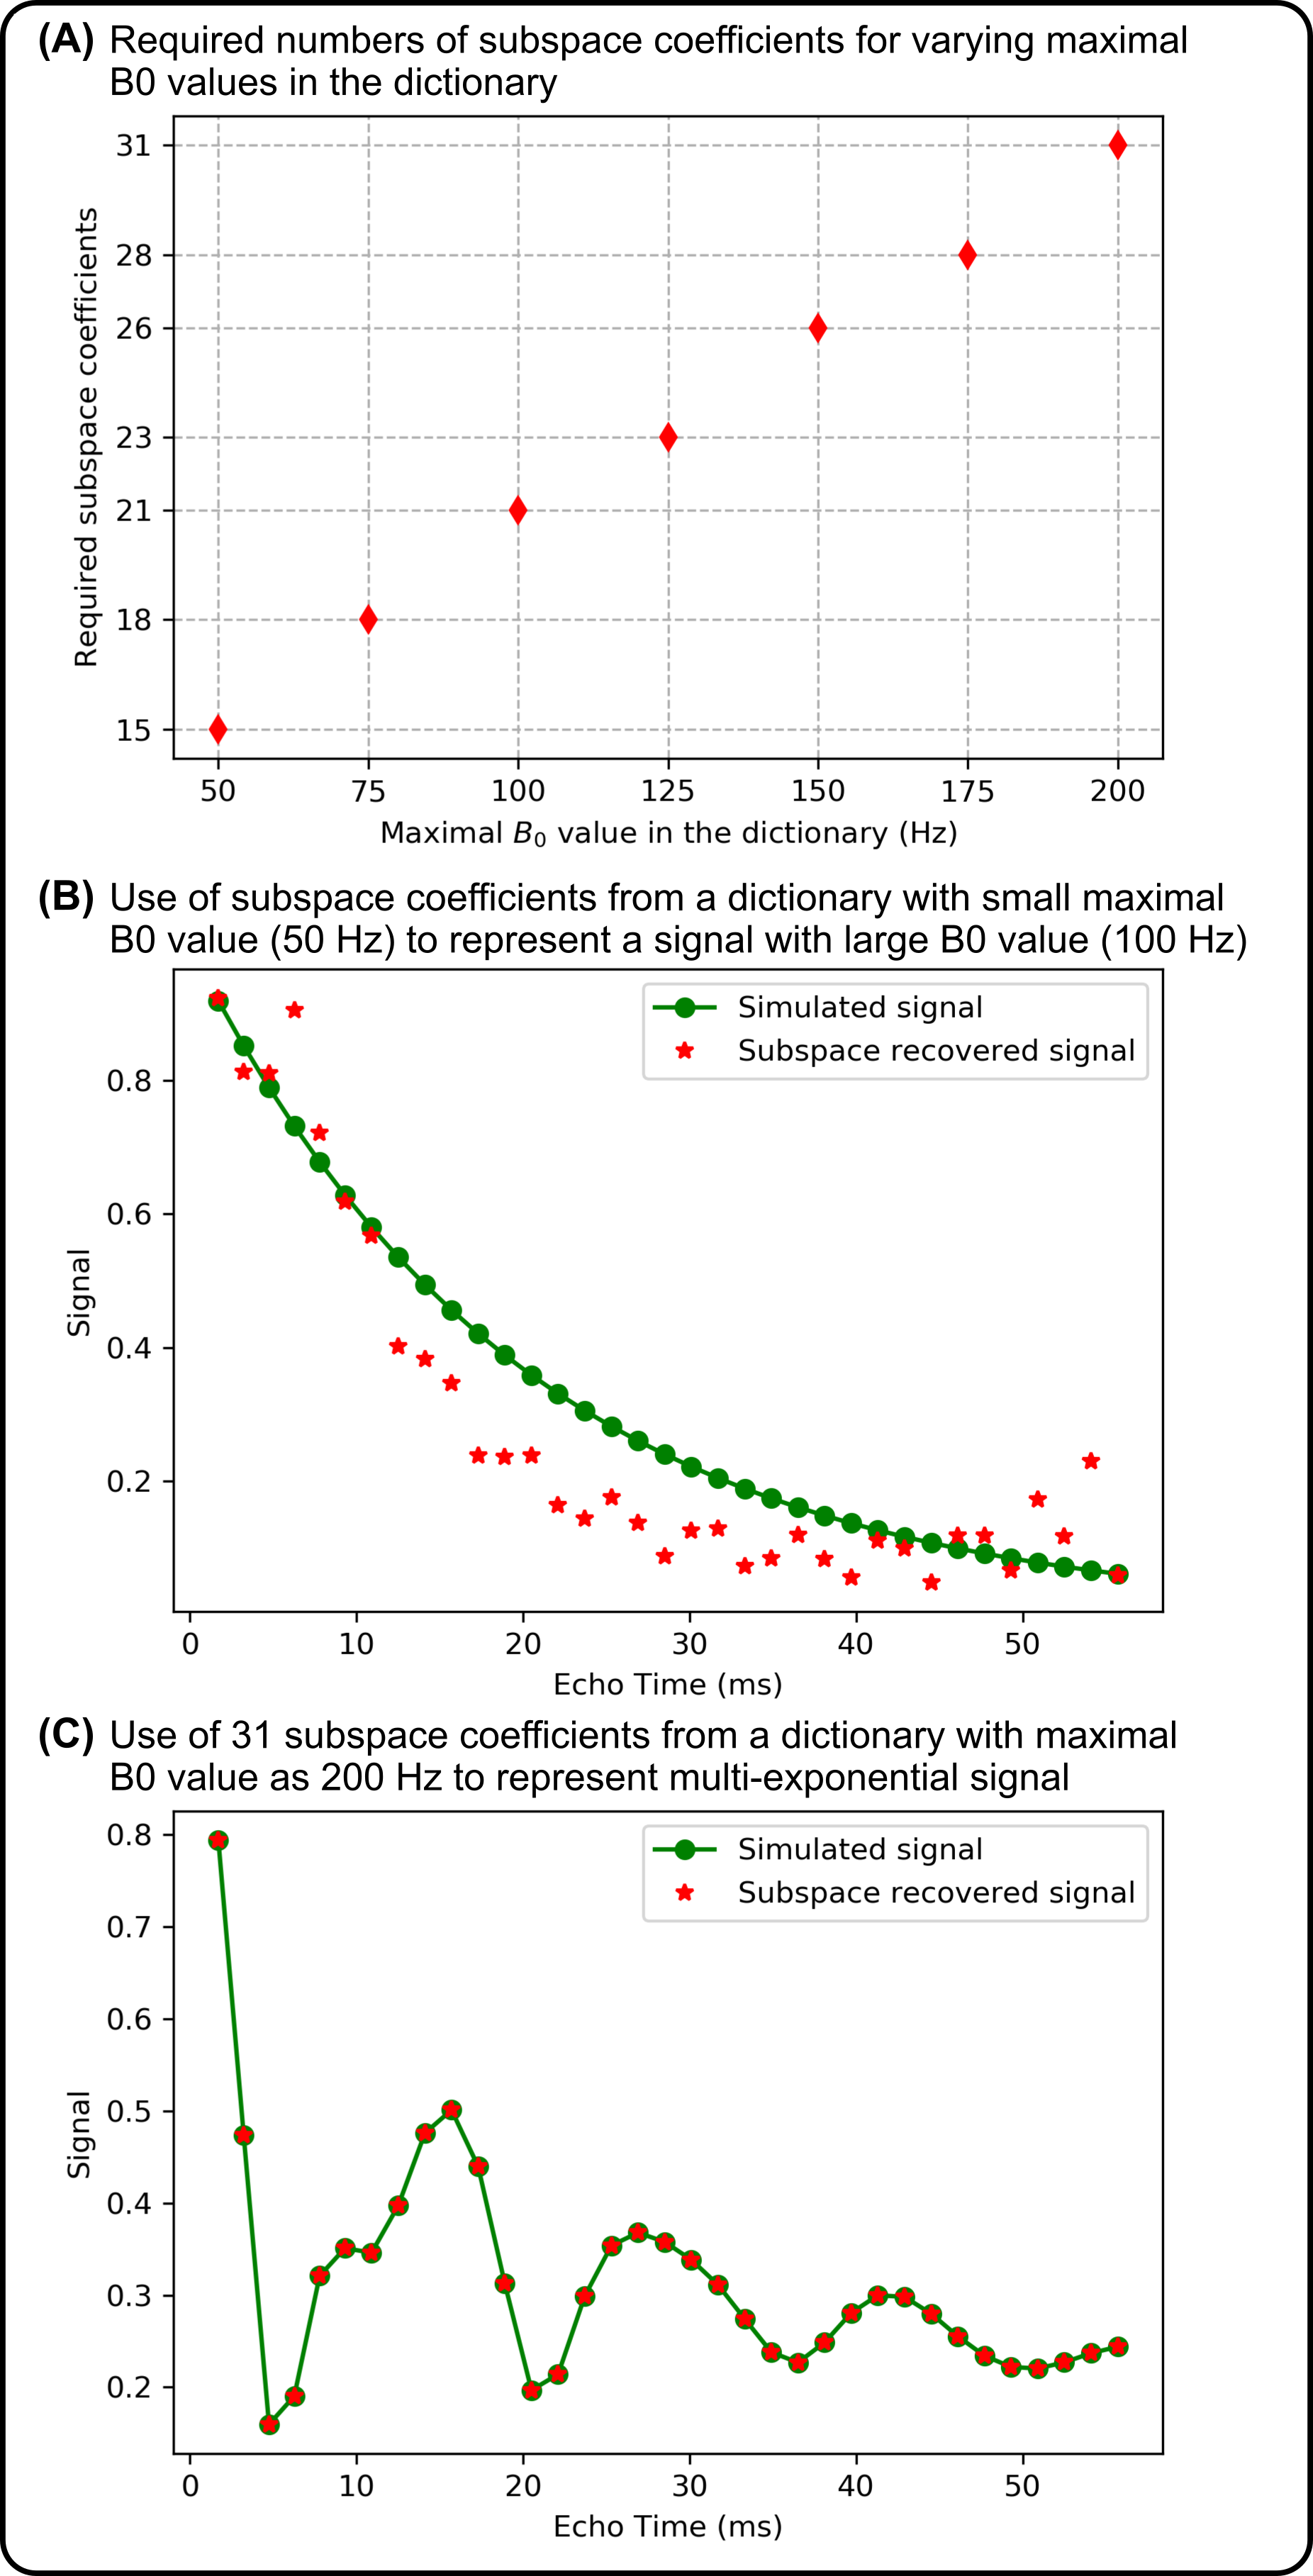
\includegraphics[width=0.6\textwidth]{../figures/fig1.png}
\fi
	\caption{Linear subspace simulations of multi-gradient-echo (MGRE) signals.
	\textbf{(A)} When increasing the maximal $B_0$ values 
	(minimum is minus maximum of $B_0$)
	in MGRE signal dictionary simulation,
	the required number of subspace coefficients increases.
	\textbf{(B)} The use of only 15 subspace coefficients from a dictionary 
	with a small maximal $B_0$ value (\SI{50}{Hz}) can not represent a signal 
	with large $B_0$ value (\SI{100}{Hz}).
	\textbf{(C)} Subspace modeling can represent multi-exponential signal. 
	The simulated signal contains 
	proton density with values \num{0.3}, \num{0.3} and \num{0.4}, 
	$T_2^*$ with values \num{20}, \num{10} and \num{100}~\si{\ms}, and 
	off-resonance frequencies with values \num{50}, \num{100} and \num{-20}~\si{\Hz}, 
	respectively.}
	\label{FIG:SubspaceSim}
\end{figure}

\ifdefined\InternRev
\pagebreak
\fi

\begin{figure}[H]
	\centering
\ifdefined\InternRev
	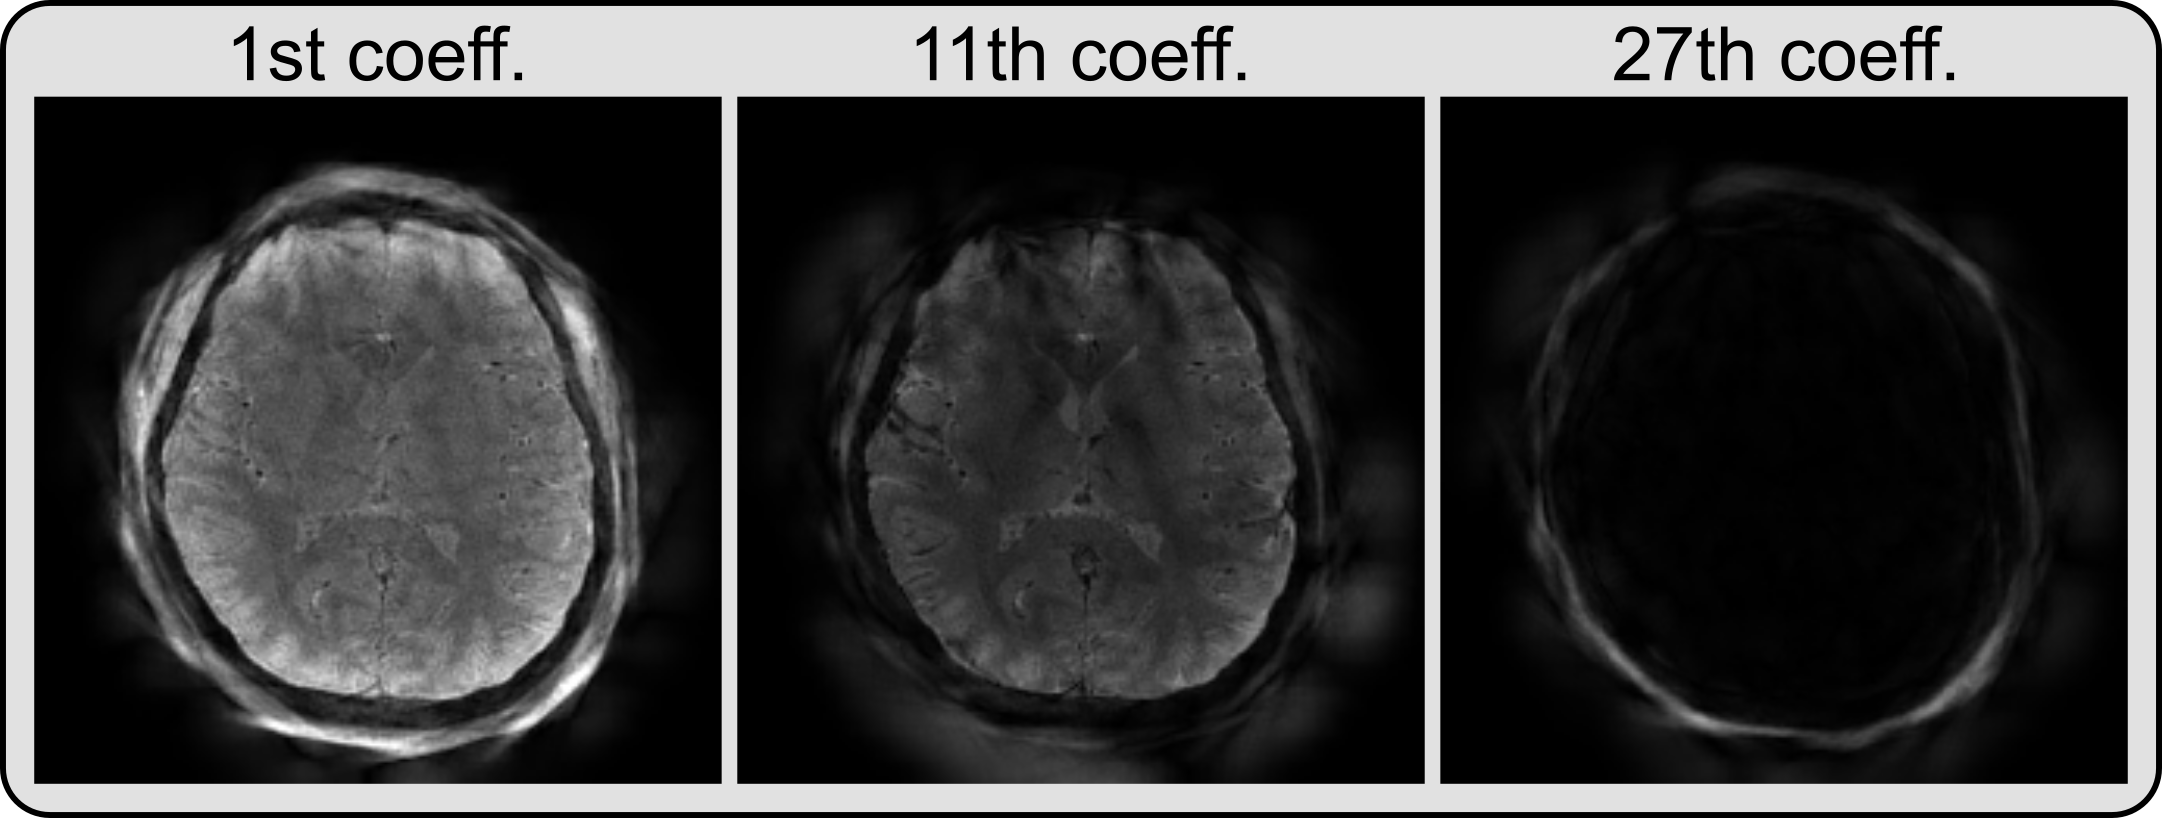
\includegraphics[width=\textwidth]{../figures/fig2.png}
\fi
	\caption{Representative subspace coefficient maps 
		from the linear subspace reconstruction. 
		In the \nth{27} coefficient, 
		only the fat layer with large off-resonance frequencies is visible.}
	\label{FIG:BasisCoef}
\end{figure}

\ifdefined\InternRev
\pagebreak
\fi

\begin{figure}[H]
	\centering
\ifdefined\InternRev
	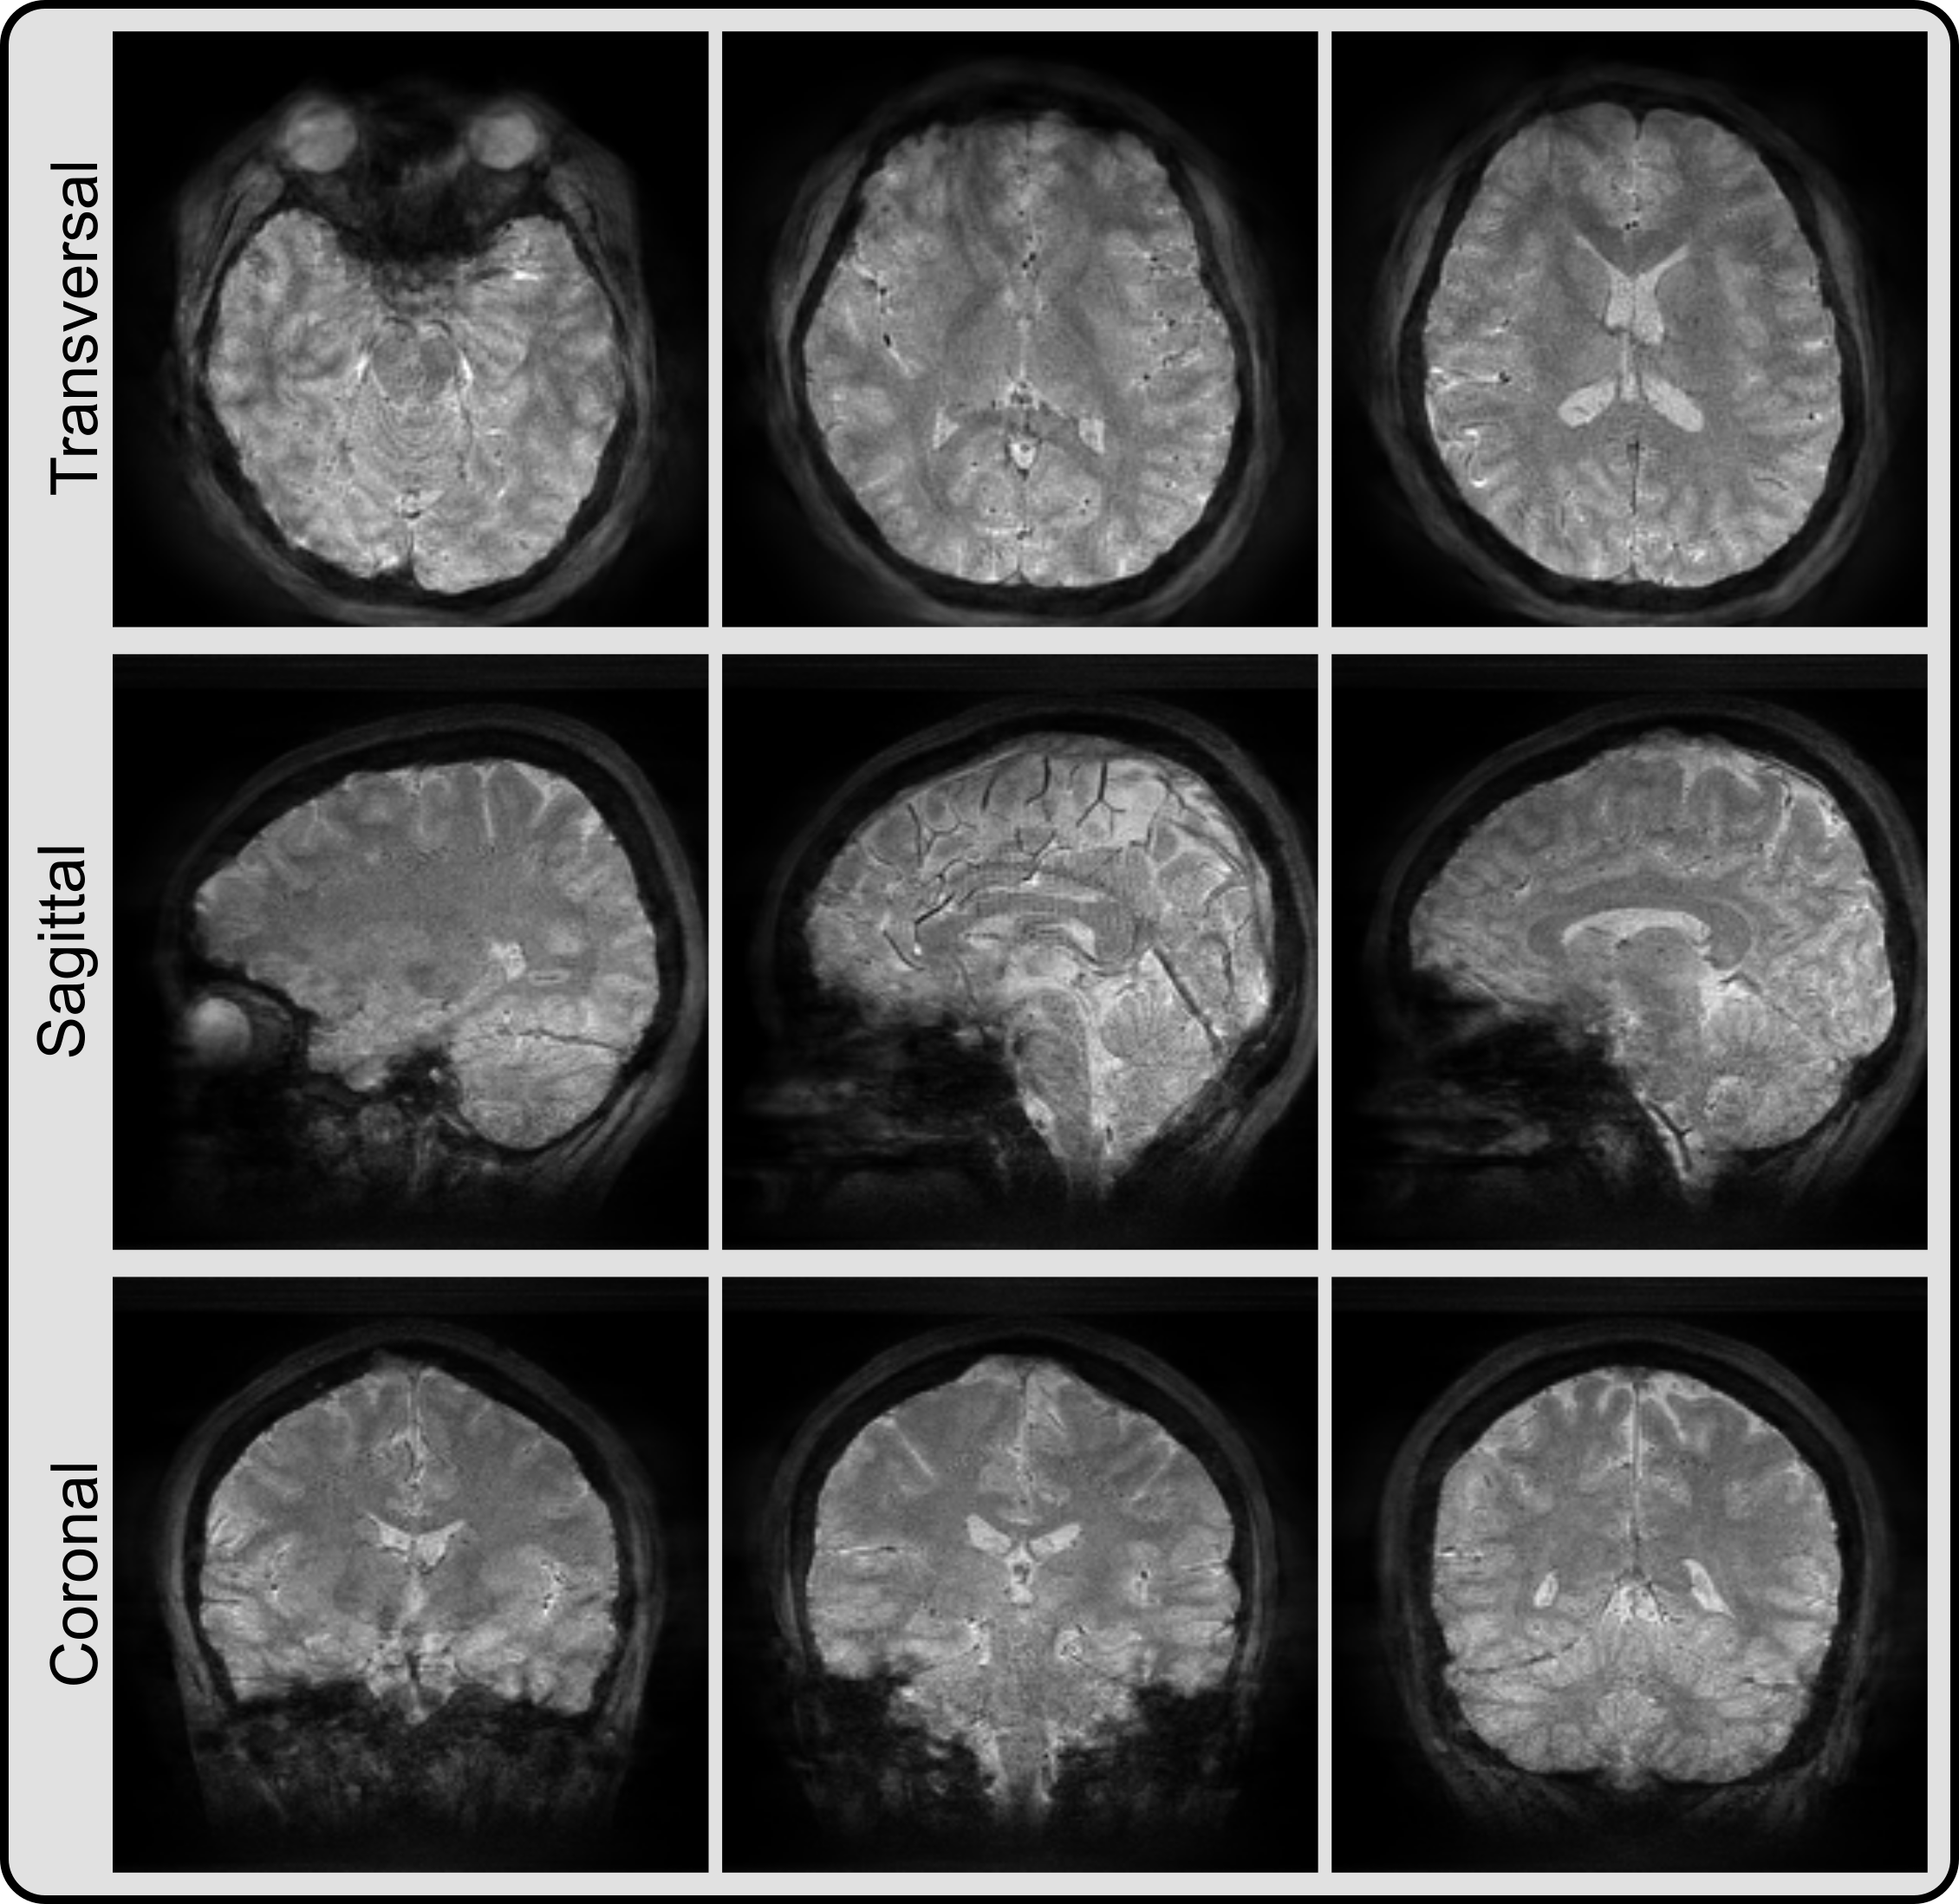
\includegraphics[width=\textwidth]{../figures/fig3.png}
\fi
	\caption{Representative slices of the echo-combined images: 
		(top) transversal, (middle) sagittal, and (bottom) coronal views.
		Three slices from every view orientation are selected for display.}
	\label{FIG:3DBrain}
\end{figure}

\ifdefined\InternRev
\pagebreak
\fi

\begin{figure}[H]
	\centering
	\ifdefined\InternRev
	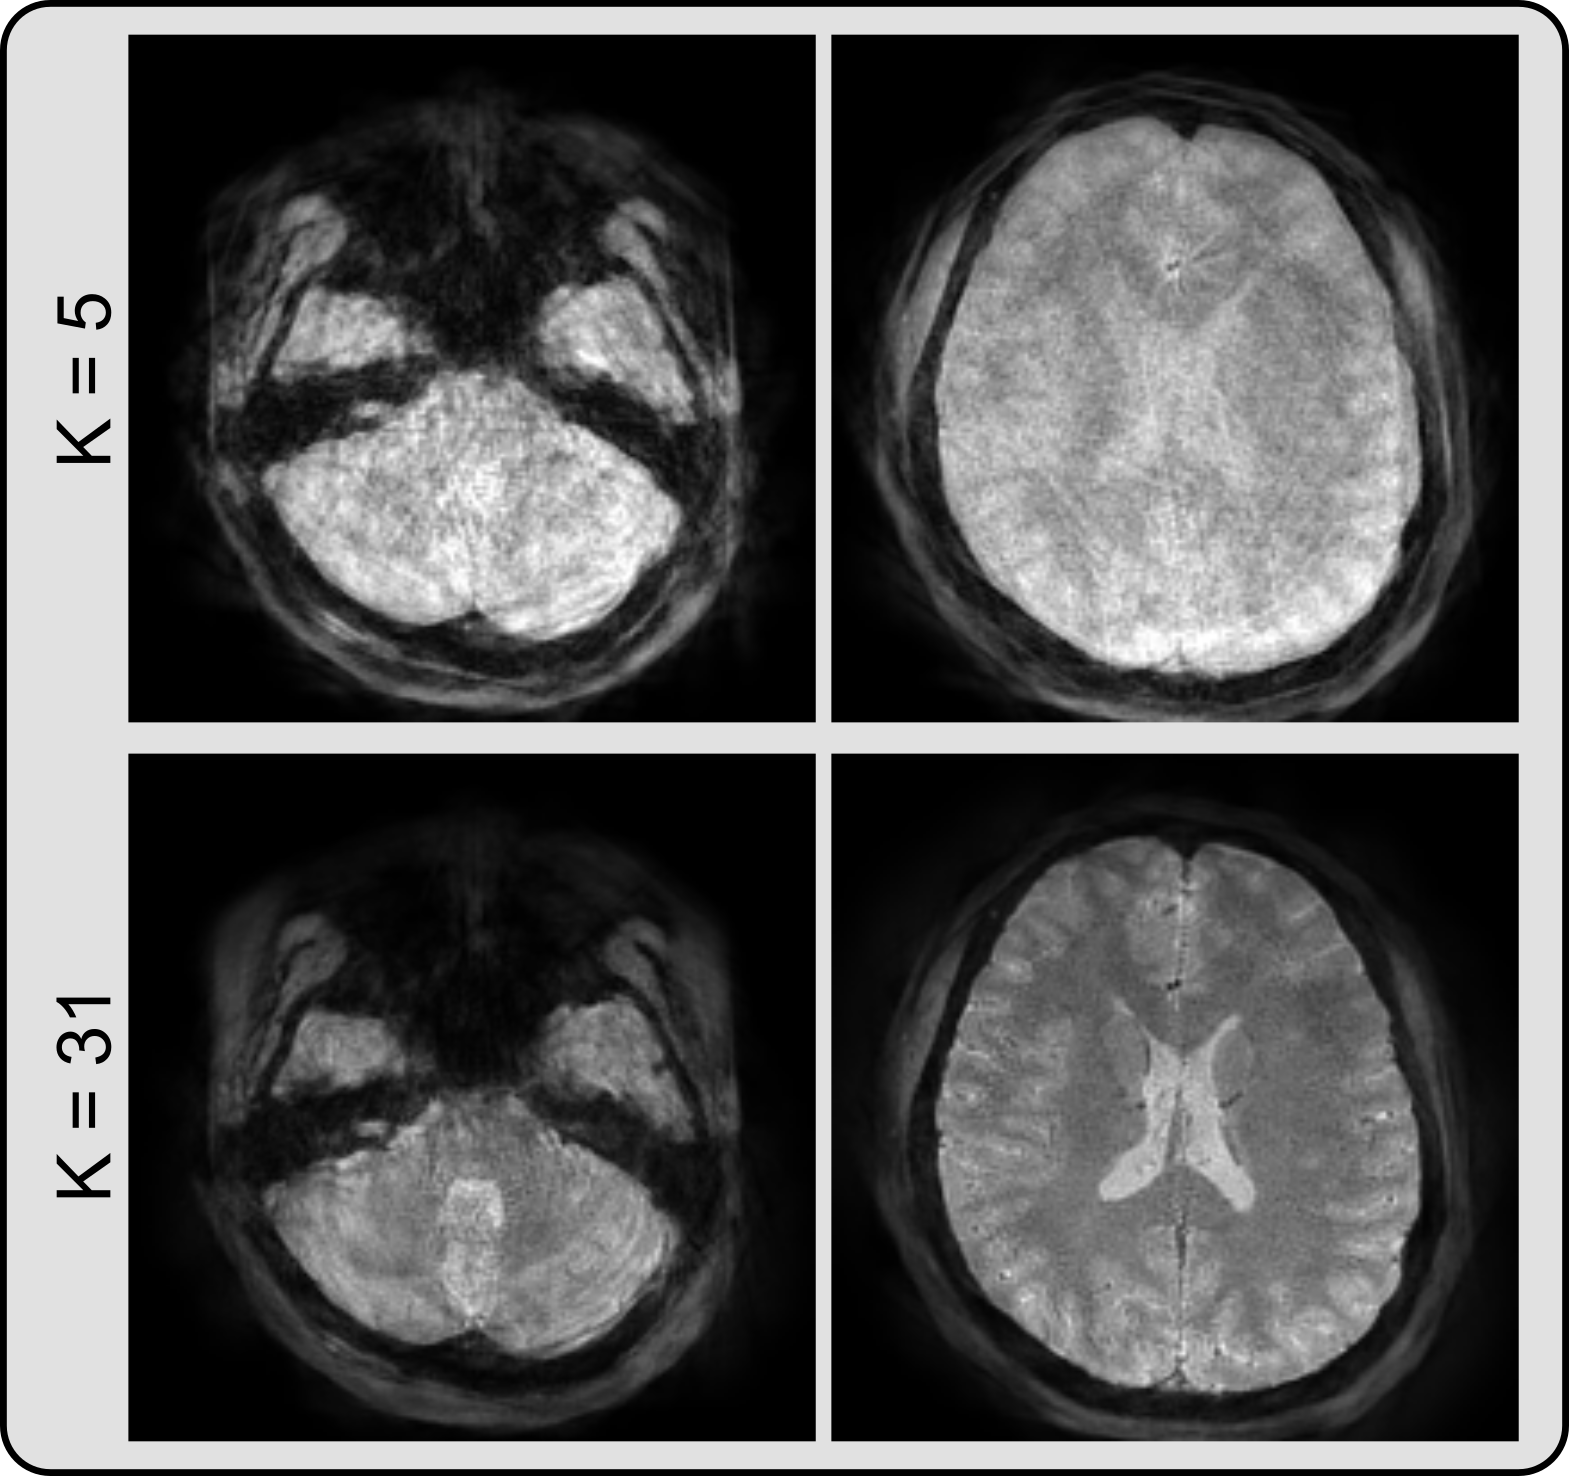
\includegraphics[width=0.7\textwidth]{../figures/fig4.png}
	\fi
	\caption{Echo-combined images from the linear subspace reconstruction 
		using (top) 5 and (bottom) 31 coefficients 
		in the truncated matrix $\hat{U}$, respectively. 
		The $B_0$ values in the dictionary is kept consistent, 
		i.e. linearly varying from \num{-100} to \SI{100}{\Hz} with \num{101} atoms.}
	\label{FIG:BasisSize}
\end{figure}

\ifdefined\InternRev
\pagebreak
\fi

\begin{figure}[H]
	\centering
	\ifdefined\InternRev
	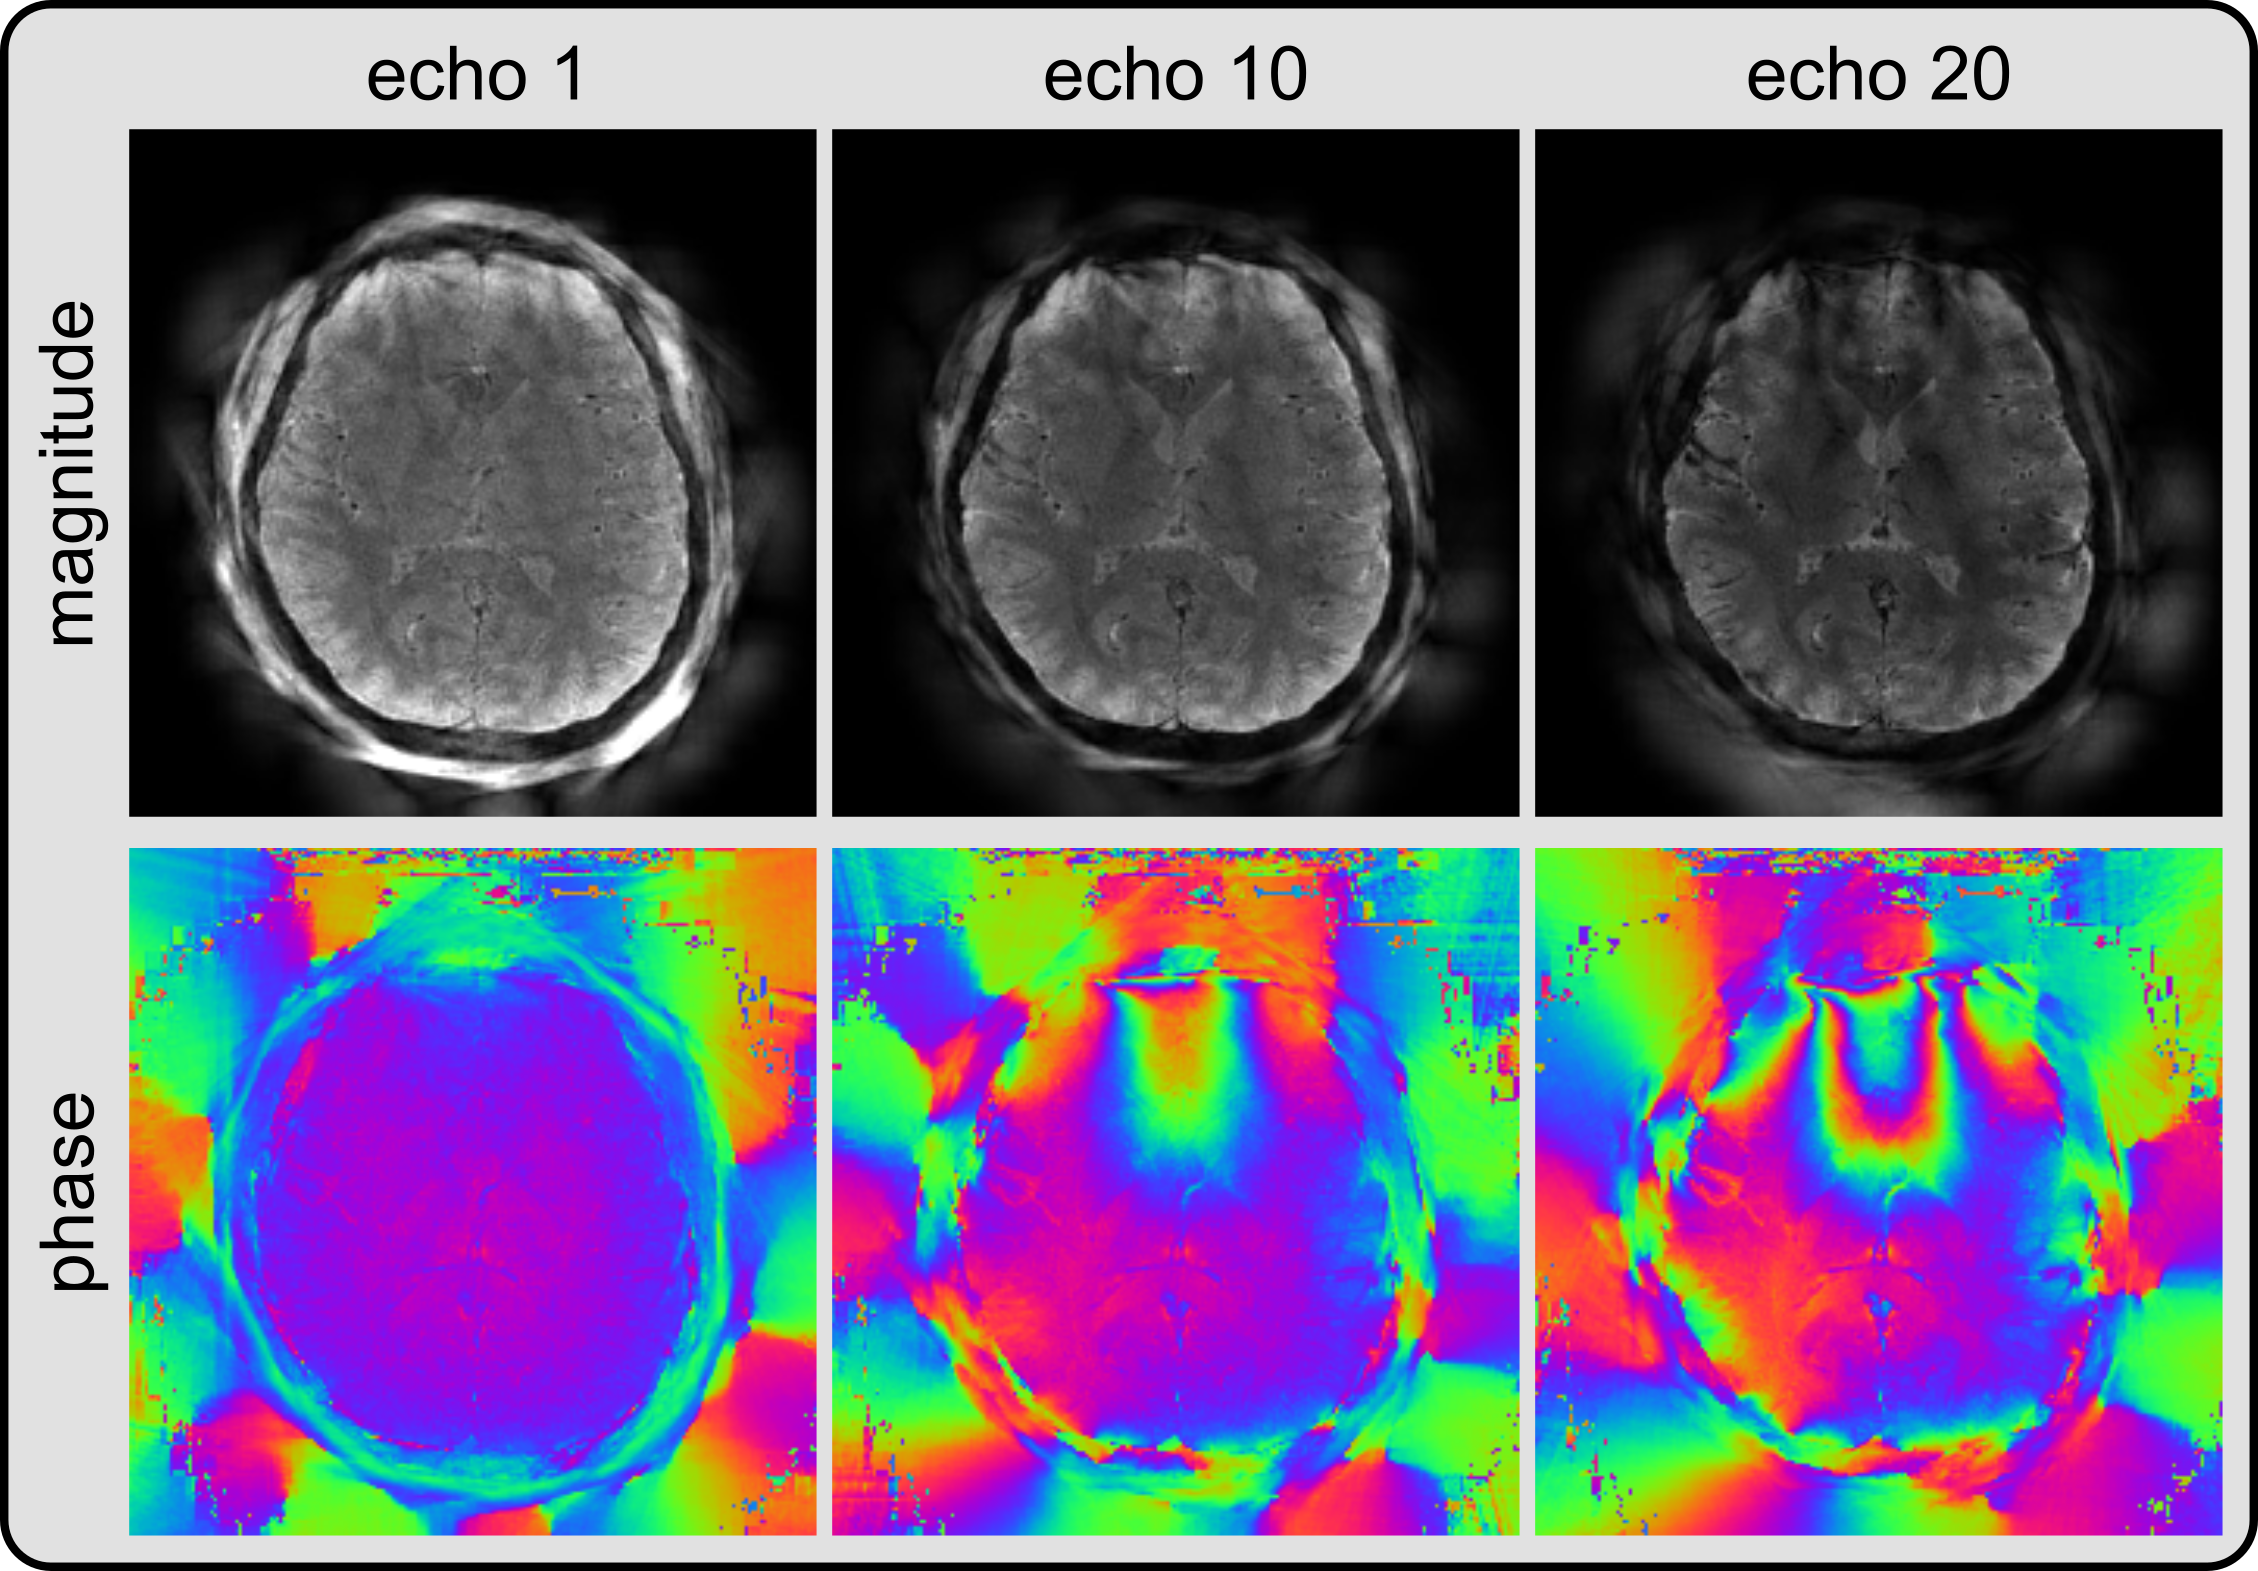
\includegraphics[width=\textwidth]{../figures/fig5.png}
	\fi
	\caption{The magnitude and phase images 
		of the \nth{1}, \nth{10}, and \nth{20} echoes 
		via linear subspace reconstruction with 
		the same dictionary as in \cref{FIG:BasisSize} and $K = 31$.}
	\label{FIG:Echoes}
\end{figure}

\pagebreak

% =============================================== %
% 		supporting information
% =============================================== %
\section*{SUPPORTING INFORMATION}

Additional Supporting Information may be found online in 
the Supporting Information section.

\vspace{2em}

\noindent \textbf{Figure S1}. (Top) Screenshot of the segmented radial EPI sequence 
implemented on Siemens pulse sequence programming platform. In this work, one complete 
$k$-space consists of seven excitation (segments). 
(Bottom) Zoomed-in sequence diagram of the third TR block. 
Note that this simulation presents the case of 2D acquisition. 
For 3D acquisition, every TR block is repeated for all $k_z$ partitions 
until the next TR block with different segment of radial spokes.

\vspace{2em}

\noindent \textbf{Figure S2}. Color-coded illustration of the radial EPI sequence 
from one excitation and its corresponding $k$-space trajectory. 
The elongated black line after the readout of the last echo 
represents the spoiling gradients.

\vspace{2em}

\noindent \textbf{Figure S3}. Adjoint NUFFT with density compensation 
reconstruction results of the same slices and orientation views 
as in \cref{FIG:3DBrain}.

\vspace{2em}

\noindent \textbf{Video S1}. The echo-combined images from the total 192 slices in three orientation views.

\end{document}
